\begin{table}
\centering
\begin{tabular}{|l|c|c|c|c|c|c|c|}
\hline
{\bf Št. glagolov} & {\bf 0} & {\bf 1} & {\bf 2} & {\bf 3} & {\bf 4} & {\bf $\geq$ 5} & {\bf $\sum$} \\
\hline
{\bf Korpus}        & 1113   & 2680   & 1019   & 164   & 18    & 6    & 5000 \\
{\bf UMDHMM}        & 2094,2 & 1691,2 & 806,8  & 288,8 & 81,4  & 37,6 & 5000 \\
{\bf Lastna impl.}  & 1865,2 & 1733,6 & 897,8  & 344,6 & 110,8 & 48   & 5000 \\
{\bf hmmlearn}      & 1898,8 & 1717,6 & 880,4  & 346,2 & 107,4 & 49,6 & 5000 \\
\hline
\end{tabular}
\caption{Porazdelitev glagolov pri izvornem besedilu in pričakovana
  porazdelitev glagolov za posamezna orodja.}
\label{tab:bench_model_table}
\end{table}

\begin{figure}
\begin{center}
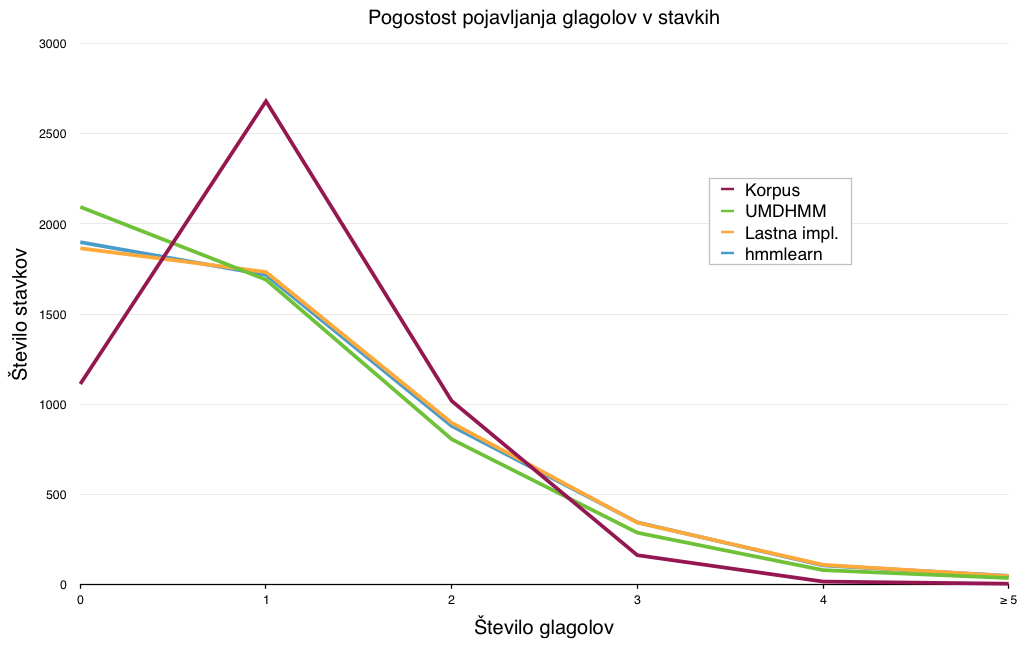
\includegraphics[width=\textwidth]{images/bench_model_comparison.png}
\end{center}
\caption{Pogostost pojavljanja glagolov pri različnih modelih.}
\label{fig:bench_model_comparison}
\end{figure}
